\documentclass{article}
\usepackage[letterpaper]{geometry}
\usepackage{fullpage}
\usepackage{amsmath}
\usepackage{amssymb}
\usepackage{graphicx}
\usepackage{wrapfig}
\usepackage{float}
\usepackage{color}
\usepackage{booktabs}
\usepackage{epstopdf}
\usepackage{subcaption}

\usepackage{fixltx2e}

\usepackage{hyperref}
\hypersetup{
    pdftitle={Sig-Fi Overview},
    pdfauthor={Joel D. Brinton},
    pdfsubject={Sig-Fi Overview},
    pdfkeywords={SigLabs, Signal Laboratories, Inc., Sig-Fi, SigFi},
    bookmarksnumbered=true,
    bookmarksopen=true,
    bookmarksopenlevel=3,
    colorlinks=true,
    pdfpagemode=UseOutlines
}
\usepackage{hypcap}

\usepackage{helvet}
\renewcommand*\familydefault{\sfdefault} %% Only if the base font of the document is to be sans serif
\usepackage[T1]{fontenc}

%\setlength({\droptitle}{-10em}



\title{\begin{center}

\includegraphics[scale=0.5]{logo2-normal-draft.eps}
\end{center}
Copper Suicide\textsuperscript{\texttrademark} User Manual\\
Scalable FPGA Development Board\\
% \subtitle{High Dynamic Range Radio with\\Split Ring Resonator-loaded MIMO Antenna}
\author{Joel D. Brinton\\Signal Laboratories, Inc.}}
% \date{July 1, 2014}

\newcommand{\designator}[1]{\textbf{\texttt{#1}}}

\begin{document}


\maketitle
\section{Abstract}

Copper Suicide is a scalable FPGA development board based on the Lattice Semiconductor ECP5 FPGA. It consists of an Arm Cortex-M7 processor, 1 configuration FPGA, 8 gigabytes of DDR3 SDRAM, and 16 general purpose FPGAs in a square 2-dimensional architecture. The design is extensible by stacking additional boards on top or bottom.

\newpage

\section{Overview}

Copper Suicide is designed to have the most flexibility between interconnections, and the highest data rate. For simplicity of design, all FPGAs have the same schematic, Figure \ref{fig:fpga} shows the FPGA interconnections. Figure \ref{fig:harness} shows the harness wiring bundles.

\begin{figure}[H]
  \centering
  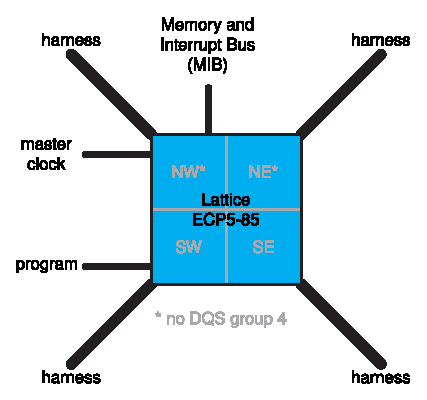
\includegraphics[scale=1]{cs_fpga.eps}
	\caption{Copper Suicide FPGA}
	\label{fig:fpga}
\end{figure}

\begin{figure}[H]
  \centering
  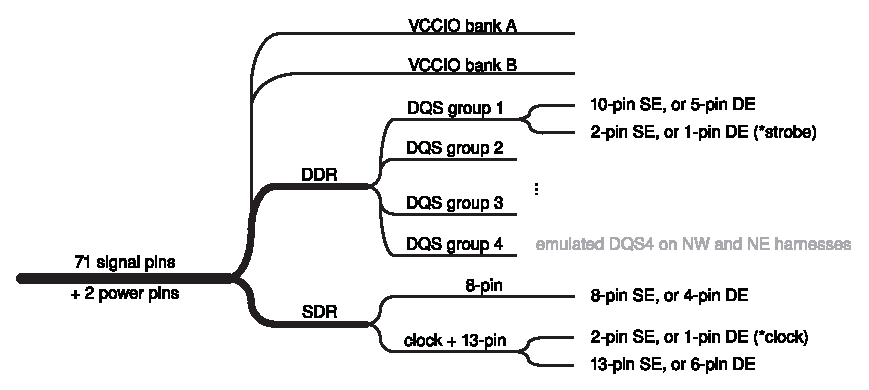
\includegraphics[scale=1]{cs_harness.eps}
	\caption{Copper Suicide Harness}
	\label{fig:harness}
\end{figure}

The FPGA block diagram, Figure \ref{fig:blockdiagram}, shows all FPGA and ARM connections.

\begin{figure}[H]
  \centering
  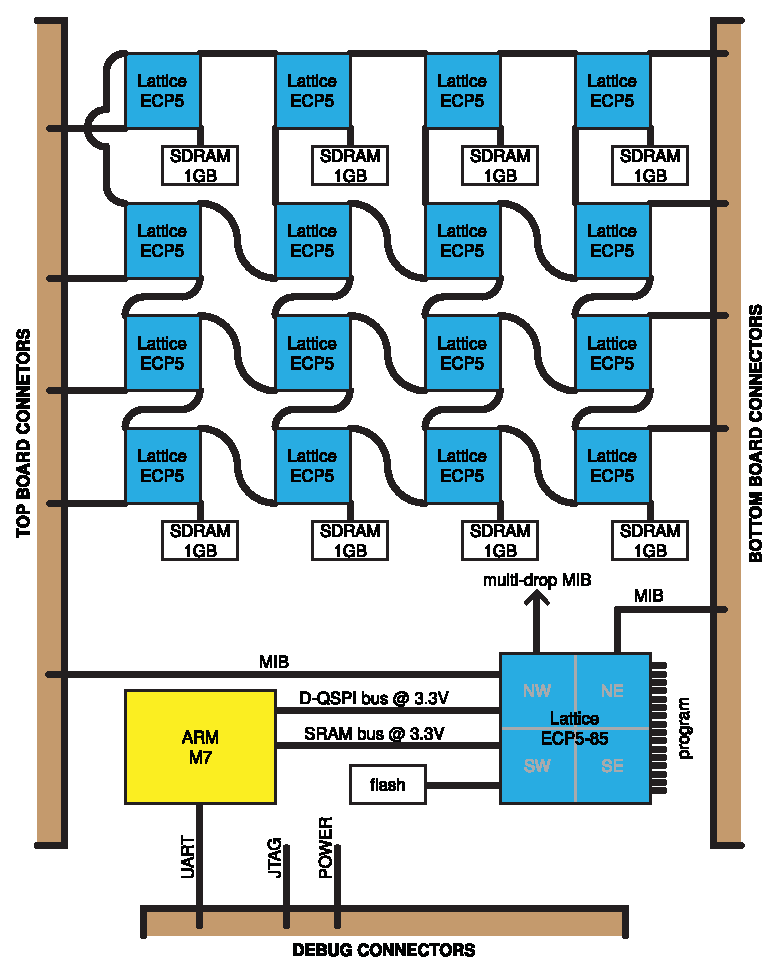
\includegraphics[scale=1]{cs_block_diagram.eps}
	\caption{Copper Suicide Block Diagram}
	\label{fig:blockdiagram}
\end{figure}

Headers...

\begin{figure}[H]
  \centering
  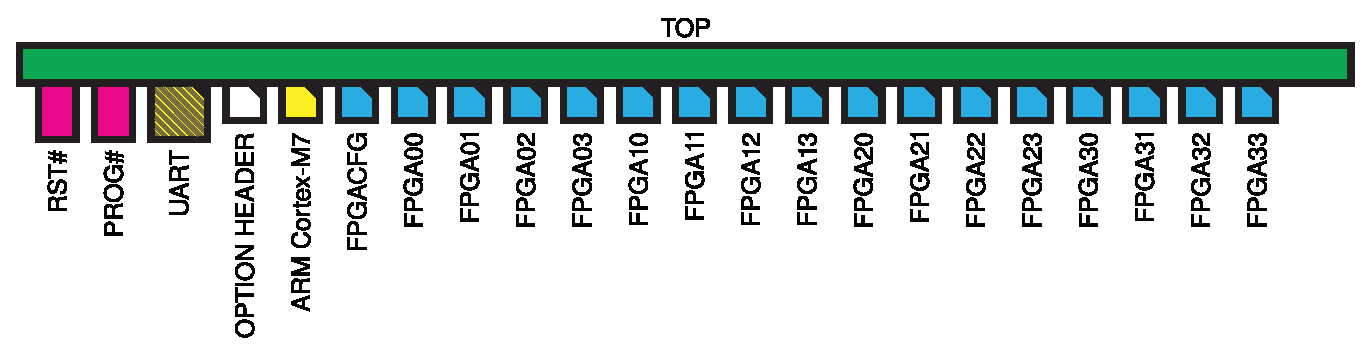
\includegraphics[scale=0.6]{cs_headers.eps}
  \caption{Copper Suicide Debug Headers}
  \label{fig:debugheaders}
\end{figure}

JTAG Connectors...

\begin{figure}[H]
  \centering
  \begin{subfigure}{0.5\textwidth}
    \centering
    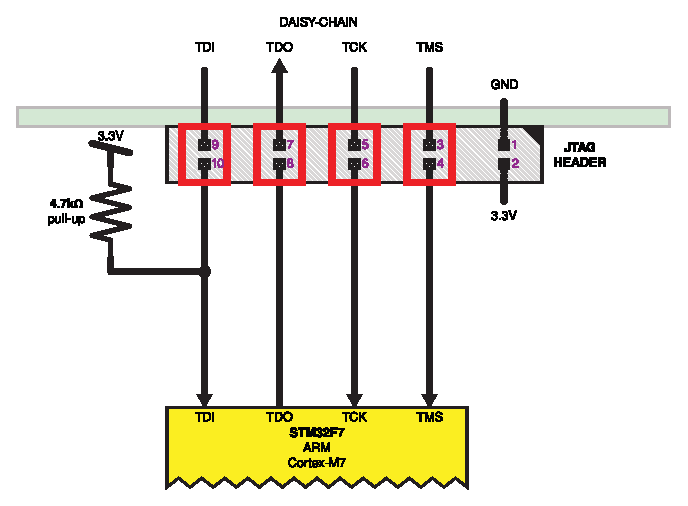
\includegraphics[width=0.8\linewidth]{cs_arm_jtag}
    \caption{ARM Cortex-M7 JTAG Header}
    \label{fig:armjtag}
  \end{subfigure}%
  \begin{subfigure}{0.5\textwidth}
    \centering
    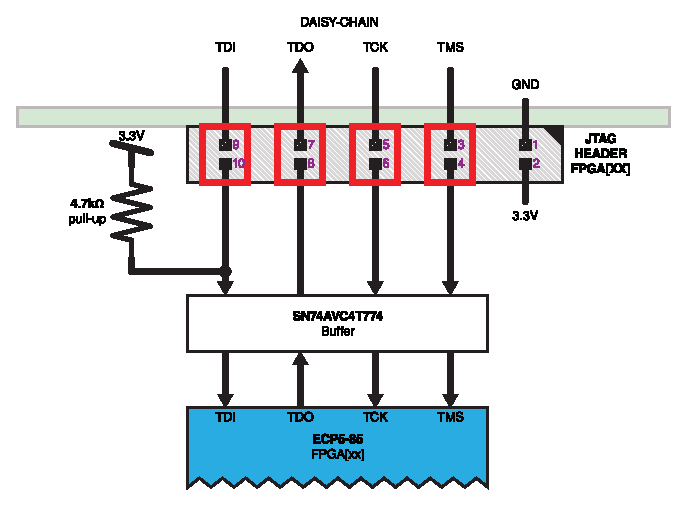
\includegraphics[width=0.8\linewidth]{cs_fpga_jtag}
    \caption{FPGA JTAG Header}
    \label{fig:fpgajtag}
  \end{subfigure}
\end{figure}

JTAG Adapter Cables

\begin{figure}[H]
  \centering
  \begin{subfigure}{0.5\textwidth}
    \centering
    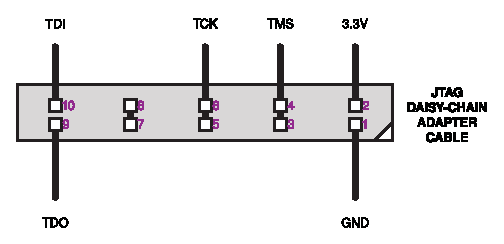
\includegraphics[width=0.8\linewidth]{cs_jtag_daisy-chain_adapter_cable}
    \caption{JTAG daisy-chain cable}
    \label{fig:jtagdaisychaincable}
  \end{subfigure}%
  \begin{subfigure}{0.5\textwidth}
    \centering
    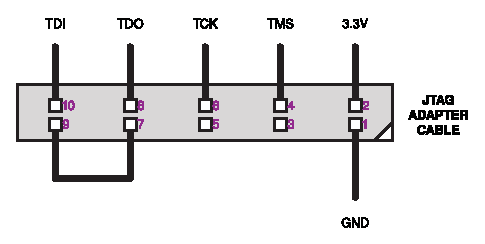
\includegraphics[width=0.8\linewidth]{cs_jtag_adapter_cable}
    \caption{JTAG cable}
    \label{fig:jtagcable}
  \end{subfigure}
\end{figure}


\newpage

\subsection{JTAG}

The JTAG daisy-chain starts at the top of the board and connects the MCU and all 17 FPGAs, figure \ref{fig:jtagdaisy}. Each device may be removed from the daisy chain with jumpers on the side of the board. If there is a need to connect to a single device the same jumpers may be used as a direct JTAG connection.

The daisy-chain may be extended to additional boards through the top and bottom connectors. For example another Copper Suicide board may be connected for a total of 36 devices in the chain. If there is no other board connected to the bottom of Copper Suicide then a jumper must be placed on \designator{P1} to connect the daisy-chain TDO to the top of the board (JTAG loopback).

Each Copper Suicide board has a TCK and TMS buffer to reduce capacitance. The TDO is a pass through 

\begin{figure}[H]
  \centering
  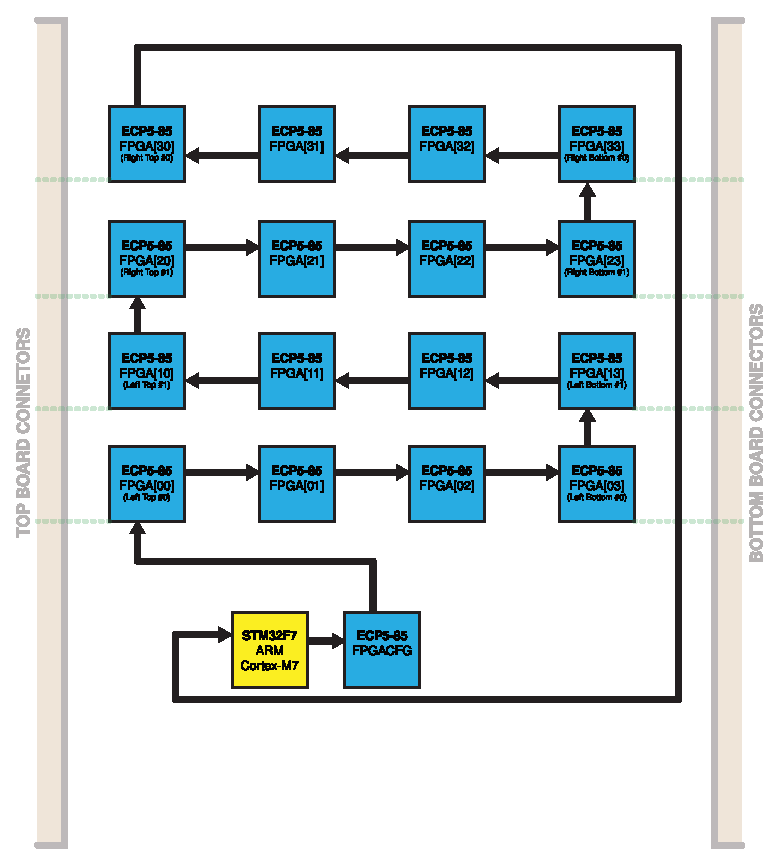
\includegraphics[scale=1]{jtag_daisy.eps}
  \caption{Copper Suicide Block Diagram}
  \label{fig:jtagdaisy}
\end{figure}

\section{Pinouts}




\end{document}
